%Example of use of oxmathproblems latex class for problem sheets
\documentclass{oxmathproblems}

%(un)comment this line to enable/disable output of any solutions in the file
%\printanswers

%define the page header/title info
\course{Algorithm Design and Analysis (Fall 2023)}
\sheettitle{Assignment 5\\Deadline: Jan 2, 2023} %can leave out if no title per sheet

\begin{document}
\begin{questions}

\miquestion[30] \textbf{[Menger's Theorem]}
Let $G=(V,E)$ be a connected undirected graph. The \emph{edge connectivity} of $s,t\in V$ is the minimum number of edges whose removal disconnects $s$ and $t$.
The \emph{vertex connectivity} of $s,t$ is the minimum number of graph elements (any vertex in $V\setminus\{s,t\}$ or any edge in $E$) whose removal disconnects $s$ and $t$. Menger's Theorem states that the edge connectivity of $s,t$ is exactly the number of edge-disjoint paths between $s$ and $t$ and the vertex connectivity of $s,t$ is exactly the number of \emph{internally} vertex-disjoint paths between $s$ and $t$. (Obviously, two paths between $s$ and $t$ are not vertex-disjoint since they intersect at $s$ and $t$; \emph{internally} vertex disjoint means they are disjoint except for $s$ and $t$.)

Prove that Menger's Theorem is just a consequence of the max-flow-min-cut theorem. Be sure the network you construct is \emph{directed} and \emph{capacitated}.

\vspace{0.5cm}
\begin{Solution}
    
First, I'll show that max edge-disjoint paths is equivalent to min edge connectivity in the connected undirected graph $G$ by applying the maxflow-mincut theorem.

Reconstruct $G$ into $G'$ as follows: replace each undirected edge $\{u, v\}$ with two directed edges $(u, v)$ and $(v, u)$, and set $c(u, v)=c(v, u)=1$. 

Following two claims imply the equivalence of four problems, and furthermore, the first part of Menger's Theorem:

\begin{enumerate}
    \item Edge-disjoint paths is equivalent to the flow. That is, $k$ edge-disjoint paths imply the existence of flow of $k$ and vice versa.
    
    On the one hand, it is trivial that $k$ edge-disjoint paths contribute $k$ units of flow by setting edges $(u, v)$ in these $k$ paths to $f(u, v)=c(u, v)=1$. On the other hand, for $k$ units of flow, we can find a path with edges $(u, v)$ with $f(u, v)=1$ and then set $f(u, v)$ to $0$, which is always possible by the definition of flow. Iteratively repeat $k$ times then we can obtain $k$ edge-disjoint paths.

    \item Edge connectivity is equivalent to the cut. That is, $k$ edge-connectivity imply the existence of cut of $k$ and vice versa.
    
    On the one hand, with $k$ edge-connectivity, we can obtain cut of $k$ by letting $L$ to be all vertices reachable from $s$ without edges in $k$ edge-connectivity, and $R$ to be the remaining vertices. Then $c(L, R)$ is exactly $k$ since $s$, $t$ are disconnected and the capacity of each edge is $1$. On the other hand, it is trivial that edges in cut of $k$ consisting $k$ edge-connectivity since $L$ and $R$ are disconnected.

    \end{enumerate}

Now, I'll show that max internally vertex-disjoint paths is equivalent to min vertex connectivity in $G$.

Reconstruct $G$ into $G'$ as follows: Split each vertex $u$ (except $s$ and $t$) into two vertices $u_{in}$, $u_{out}$ and an directed edge $(u_{in}, u_{out})$ with $c(u_{in}, u_{out})=1$, transform each undirected edge $\{u, v\}$ into two directed edges $(u_{out}, v_{in})$, $(v_{out}, u_{in})$ with capacity of $\infty$. 

Similar to the previous part, following two claims imply the second part of Menger's Theorem: 

\begin{enumerate}
    \item Internally vertex-disjoint paths is equivalent to the flow. That is, $k$ internal vertex-disjoint paths imply the existence of flow of $k$ and vice versa.
    
    The proof is same to that of previous part, instead $c(u_{in}, u_{out})=1$ constraints the flow of each path to be $0$ or $1$.

    \item Vertex connectivity is equivalent to the cut. That is, $k$ vertex-connectivity imply the existence of cut of $k$ and vice versa.
    
    First, we can make some adjustments to ensure that vertex connectivity only contains edges like $(u_{in}, u_{out})$ (i.e., edges reconstructed from a single vertex): if there exists edges $(u_{out}, v_{in})$, $u\neq v$ in vertex connectivity, we can replace them with either endpoints ($(u_{in}, u_{out}$ or $(v_{in}, v_{out})$ in $G'$) while maintaining the graph disconnected. Left part is same to the proof of the second claim of previous part.
\end{enumerate}
    
\end{Solution}
\vspace{0.5cm}
\begin{Reference}

\href{https://www.cs.cornell.edu/courses/cs6820/2019fa/handouts/maxflow-mincut.pdf}{https://www.cs.cornell.edu/courses/cs6820/2019fa/handouts/maxflow-mincut.pdf}
\end{Reference}
\newpage

\miquestion[30] \textbf{[Perfect Matching on Bipartite Graph]}
A graph is \emph{regular} if every vertex has the same degree.
Let $G=(A,B,E)$ be a regular bipartite graph with $|E|>0$.
\begin{parts}
\part[10] Prove that $|A|=|B|$.
\part[15] Let $n=|A|=|B|$. Can we conclude that $G$ must contain a matching of size $n$? If so, prove it; if not, provide a counterexample.
\end{parts}

\begin{Solution}

\begin{parts}
    \part Let $deg(S)$ denotes the sum of degree of vertices in set $S$. Since $G=(A, B, E)$ is a bipartite graph, for any edge $e\in E$, there must be one of its endpoint in $A$ and another in $B$. Therefore, $deg(A)=deg(B)$ holds. 
    
    For the other hand, $G$ is regular, which implies each vertex has the same degree $d$. Therefore, $deg(A)=\sum_{u\in A}d=|A|d$, $deg(B)=\sum_{u\in B}d=|B|d$.

    Combining the above two conclusions, we have $|A|=|B|$.

    \part According to the conclusion introduced in the lecture and proven in next problem, \textit{maximum matching} is equal in size to \textit{minimum vertex cover} on bipartite graphs. I'll prove that the size of minimum vertex cover of $G$ is exactly $n$. Then the size of maximum matching of $G$ is also $n$, which implies the existence of matching of size $n$.

    On the one hand, the size of minimum vertex cover of $G$ is less than or equal to $n$. This goes trivial because $A$ (or $B$) with size of $n$ is one of valid vertex covers since any edge in bipartite graph $G=(A, B, E)$ has exactly one endpoint in $A$ and another in $B$.

    On the other hand, the size of minimum vertex of $G$ is greater than or equal to $n$. According to the previous part, $|E|=|A|d$. To cover all edges, the best case is each vertex covers $d$ edges without overlap. Therefore, it requires at least $|E|/d=|A|=n$ vertices.

    Therefore, the size of minimum vertex cover is exactly $n$, and we're done.
    
\end{parts}

\end{Solution}

\miquestion[40]\textbf{[K\"{o}nig-Egerv\'{a}ry Theorem]}
In the class, we have seen that the maximum matching problem can be formulated by the following linear program
\begin{align*}
\text{maximize }& \sum_{e\in E}x_e \\
\text{subject to }&\sum_{e:e=(u,v)}x_e\leq 1  \tag{$\forall v\in V$}\\
&x_e\geq0\tag{$\forall e\in E$}
\end{align*}
and the minimum vertex cover problem can be formulated by the following linear program
\begin{align*}
\text{minimize }& \sum_{u\in V}x_u \\
\text{subject to }&x_u+x_v\geq 1  \tag{$\forall (u,v)\in E$}\\
&x_u\geq0\tag{$\forall u\in V$}
\end{align*}
We have also seen that the second linear program is the dual program of the first.
\begin{parts}
\part[20] Prove that both linear programs have integral optimal solutions if the graph is bipartite.
\part[10] Using the result in the first part, prove K\"{o}nig-Egerv\'{a}ry Theorem, which states that the size of the maximum matching equals to the size of the minimum vertex cover in a bipartite graph.
\part[10] Provide a counterexample showing that the claim fails for non-bipartite graphs.
\end{parts}

\begin{Solution}
\begin{parts}
\part Let $A_1\in\mathbf{R}^{(|V|+|E|)\times|E|}$ denotes the constraint matrix of maximum matching, and $A_2\in\mathbf{R}^{(|E|+|V|)\times|V|}$ denotes that of minimum vertex cover. $A_1$ can be decomposed into $[X,\  I_1]^T$ and $A_2$ can be decomposed into $[X^T,\  I_2]^T$, where $X\in\mathbf{R}^{|V|\times|E|}$, $I_1\in\mathbf{R}^{|E|\times|E|}$ and $I_2\in\mathbf{R}^{|V|\times|V|}$. Suppose $X_{ij}$ corresponds to vertex $s$ and edge $\{u, v\}$. $X_{ij}=1$ if $s$ is one of the endpoint of $\{u, v\}$, and $X_{ij}=0$ otherwise. 

To show both linear programs have integral optimal solutions, we only need to show both $A_1$ and $A_2$ are totally unimodular. Based on the properties of totally unimodular, we only need to show $X$ is totally unimodular. By the definition, claim that every square submatrix of $X$ has determinants belonging to $\{0,\ -1,\ 1\}$. I'll show this by induction. 

\textit{\textbf{Base step:}}

Each element of $X$ is either 0 or 1, belonging to $\{0,\ -1,\ 1\}$.

\textit{\textbf{Inductive step:}}

Suppose every $k\times k$ submatrix of $X$ has determinants belonging to $\{0,\ 1,\ -1\}$. Consider any $(k+1)\times(k+1)$ submatrix $X'$. Since an edge has only two endpoints, we know that for any column of $X$, there are exactly two entries of $1$, and others are $0$. Therefore, there are three scenarios here:

\begin{enumerate}
    \item If a column of $X'$ is all-zeros, then $\det(X')=0$.

    \item If a column of $X'$ contains only one entry of $1$, then $\det(X')$ equals to the determinant of a $k\times k$ submatrix. Then $\det(X')\in\{0,\ -1,\ 1\}$.

    \item If every column of $X'$ has two entries of $1$, then for any edge in $X'$, both of the endpoints are in $X'$, which means $X'$ defines a sub-bipartite graph. Multiply rows whose corresponding vertices are in the left side of the bipartite graph by $1$, multiply other rows by $-1$, and add them all. Then we can obtain a all-zeros vector by the nature of the bipartite graph. This implies $X'$ is not linear independent, and  $\det(X')=0\in\{0,\ -1,\ 1\}$.
\end{enumerate}

\part First, it is easy to check the second linear program is the dual program of the first one. Second, according to the problem description, we know that these two linear programs describes the fractional version of maximum matching  and minimum vertex cover respectively. Third, from the previous part, we know that both linear programs have integral optimal solutions on the bipartite graph.

By the LP-duality Theorem, the primal LP optimal solution $|\{x_e^*\}|$ equals to dual LP optimal solution $|\{x_u^*\}|$, which implies  K\"{o}nig-Egerv\'{a}ry Theorem.

\part Consider the following triangle. The  size of maximum matching is $1$ (for example $\{AB\}$), but the size of minimum vertex cover is $2$ (for example $\{A, C\}$).

\begin{figure}[H]
    \centering
    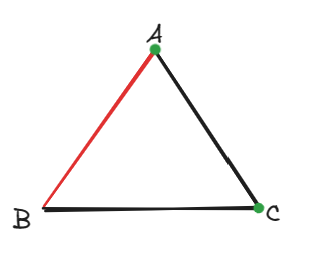
\includegraphics[width=0.25\linewidth]{image.png}
    \caption{A counterexample.}
    \label{fig:enter-label}
\end{figure}
    
\end{parts}
\end{Solution}

\miquestion[Bonus 60]
\textbf{[Dinic's Algorithm]}
In this question, we are going to work out \emph{Dinic's algorithm} for computing a maximum flow.
Similar to Edmonds-Karp algorithm, in each iteration of Dinic's algorithm, we update the flow $f$ by increasing its value and then update the residual network $G^f$.
However, in Dinic's algorithm, we push flow along \emph{multiple} $s$-$t$ paths in the residual network instead of a \emph{single} $s$-$t$ path as it is in Edmonds-Karp algorithm.

In each iteration of the algorithm, we find the \emph{level graph} of the residual network $G^f$.
Given a graph $G$ with a source vertex $s$, its level graph $\overline{G}$ is defined by removing edges from $G$ such that only edges pointing from level $i$ to level $i+1$ are kept, where vertices at level $i$ are those vertices at distance $i$ from the source $s$.
An example of level graph is shown in Fig.~\ref{fig:levelgraph}.

Next, the algorithm finds a \emph{blocking flow} on the level graph $\overline{G}^f$ of the residual network $G^f$.
A blocking flow $f$ in $G$ is a flow such that each $s$-$t$ path contains at least one \emph{critical edge}.
Recall that an edge $e$ is \emph{critical} if the amount of flow on it reaches its capacity: $f(e)=c(e)$.
Fig.~\ref{fig:blockingflow} gives examples for blocking flow.

Dinic's algorithm is then described as follows.
\begin{enumerate}
    \item Initialize $f$ to be the empty flow, and $G^f=G$.
    \item Do the following until there is no $s$-$t$ path in $G^f$:
    \begin{itemize}
        \item construct the level graph $\overline{G}^f$ of $G^f$.
        \item find a blocking flow on $\overline{G}^f$.
        \item Update $f$ by adding the blocking flow to it, and update $G^f$.
    \end{itemize}
\end{enumerate}

\begin{figure}[htbp]
    \centering
    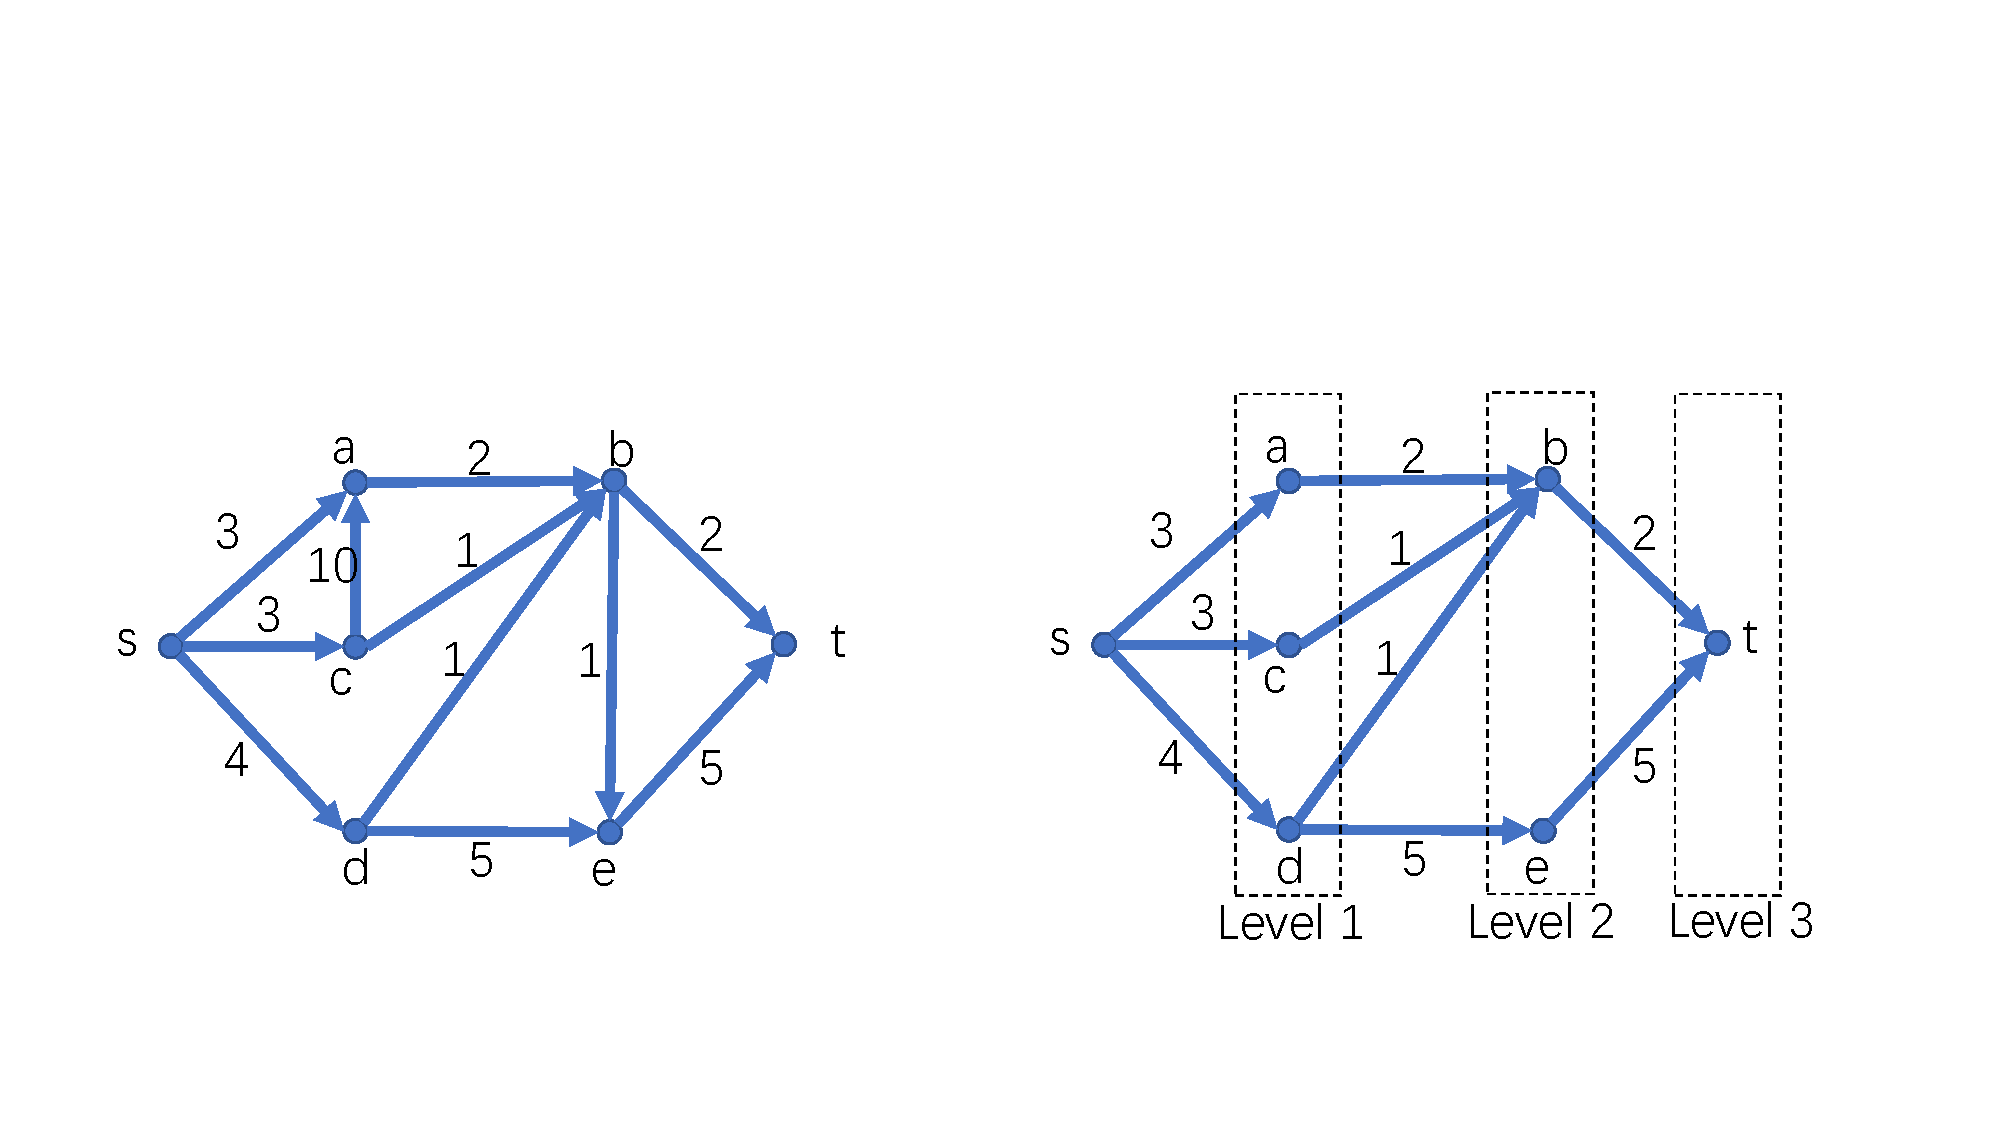
\includegraphics[width=\textwidth]{levelgraph.pdf}
    \caption{The graph shown on the right-hand side is the level graph of the graph on the left-hand side. Only edges pointing to the next levels are kept. For example, the edges $(c,a)$ and $(b,e)$ are removed, as they point at vertices at the same level. If there were edges pointing at previous levels, they should also be removed.}
    \label{fig:levelgraph}
\end{figure}

\begin{figure}[htbp]
    \centering
    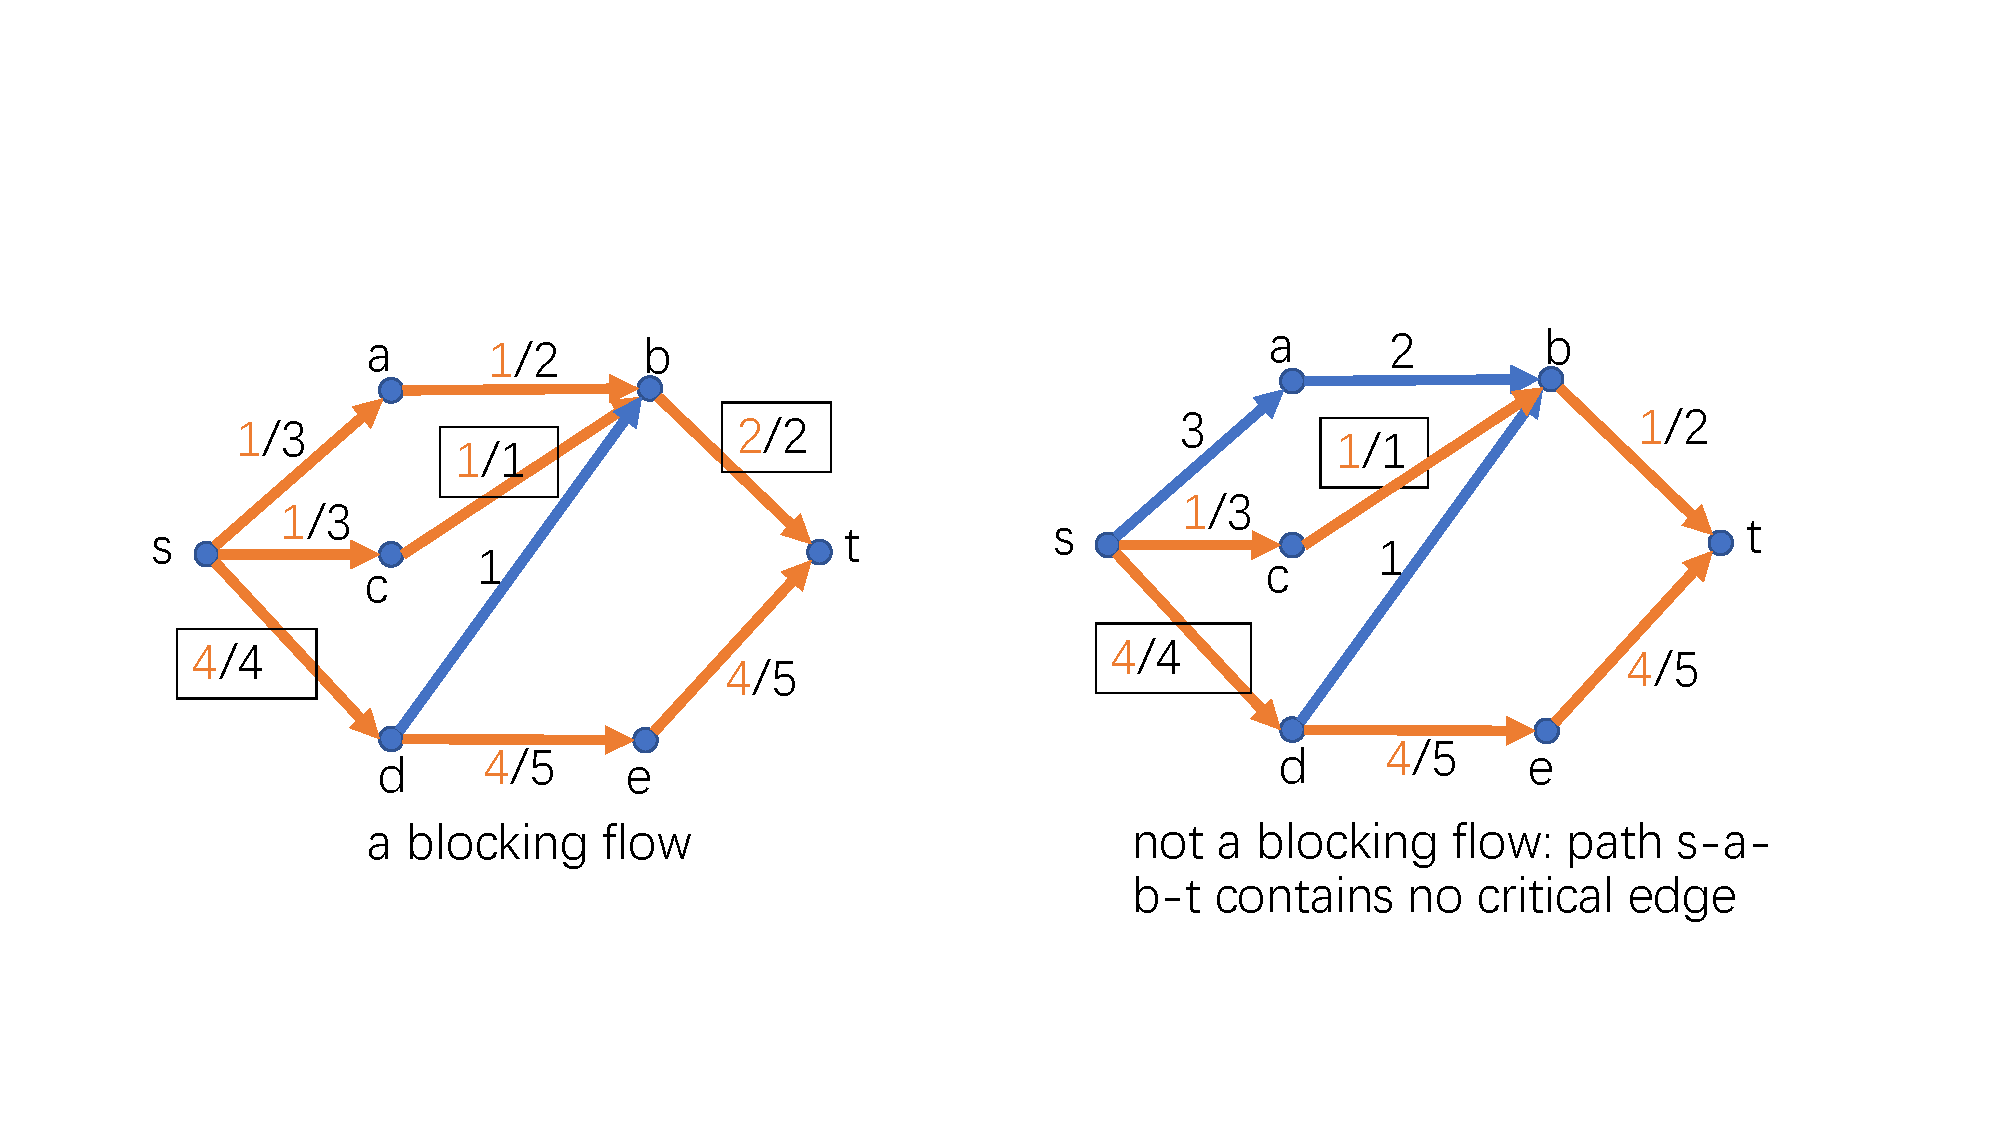
\includegraphics[width=\textwidth]{blockingflow.pdf}
    \caption{Blocking flow examples}
    \label{fig:blockingflow}
\end{figure}

Complete the analysis of Dinic's algorithm by solving the following questions.
\begin{parts}
\part[15] Prove that, after each iteration of Dinic's algorithm, the distance from $s$ to $t$ in $G^f$ is increased by at least $1$.
\part[15] Design an $O(|V|\cdot |E|)$ time algorithm to compute a blocking flow on a level graph.
\part[10] Show that the overall time complexity for Dinic's algorithm is $O(|V|^2\cdot|E|)$.
\part[20] \textbf{(challenging)} We have seen in the class that the problem of finding a maximum matching on a bipartite graph can be converted to the maximum flow problem. Show that Dinic's algorithm applied to finding a maximum matching on a bipartite graph only requires time complexity $O(|E|\cdot\sqrt{|V|})$.
\end{parts}

\miquestion
How long does it take you to finish the assignment (including thinking and discussion)?
Give a score (1,2,3,4,5) to the difficulty.
Do you have any collaborators?
Please write down their names here.

\end{questions}

\begin{Solution}

These three questions cost 3.5h, 2h, 3h respectively (typing also included).

The difficulty scores are 3, 2, 3 respectively.
\end{Solution}
\end{document}
